%%%%%%%%%%%%%%%%%%%%%%%%%%%%%%%%%%%%%%%%%%%%%%%%%%%%%%%%%%%%%%%%%%%%%%
% Prosojnice za predstavitev seminarja (skupina 16, NPMP 2026/2027)
% Prevajanje: latexmk -pdf prosojnice.tex   (v mapi prosojnice/)
% Slike so iste kot v porocilu: ../porocilo/Skupina16/img/
%%%%%%%%%%%%%%%%%%%%%%%%%%%%%%%%%%%%%%%%%%%%%%%%%%%%%%%%%%%%%%%%%%%%%%

\documentclass[aspectratio=169, 11pt]{beamer}
\usetheme[progressbar=frametitle, numbering=fraction]{metropolis}

\usepackage[utf8]{inputenc}
\usepackage[T1]{fontenc}
\usepackage[slovene]{babel}
\usepackage{amsmath}
\usepackage{physics}
\usepackage{booktabs}
\usepackage[separate-uncertainty=true]{siunitx}
\sisetup{output-decimal-marker={,}}
\usepackage{tikz}
\usepackage{quantikz}

\graphicspath{{../porocilo/Skupina16/img/}}

\title{Kje Groverjev algoritem preneha delovati na IBM Heron?}
\subtitle{Napoved praga z digitalnim dvojčkom iz kalibracijskih podatkov}
\author{Gašper Jug}
\institute{Skupina 16 \quad·\quad NPMP 2026/2027}
\date{}

\begin{document}

\maketitle

% ---------------------------------------------------------------------
\begin{frame}{Vprašanje}
  \begin{itemize}
    \item Pri kolikšnem številu kubitov $n$ Groverjev algoritem na procesorju \texttt{ibm\_marrakesh} (IBM Heron, 156 kubitov) ne da več uporabnega rezultata?
    \item Ali ta prag napove \alert{digitalni dvojček}: šumni simulator, zgrajen iz kalibracijskih podatkov procesorja?
  \end{itemize}

  \vspace{1em}
  \textbf{Uporaben rezultat:} verjetnost uspeha vsaj dvakrat večja od naključnega ugibanja,
  \[
    P \geq \frac{2}{2^n}.
  \]

  \textbf{Hipoteza:} prag pri $n^* = 5 \pm 1$; dvojček ga napove, verjetnost uspeha pa preceni.
\end{frame}

% ---------------------------------------------------------------------
\begin{frame}{Groverjevo vezje}
  \centering
  \begin{quantikz}[column sep=0.22cm, row sep=0.15cm]
    \lstick{$q_0$} & \gate{H} & \gate{X} & \ctrl{1}  & \gate{X} & \gate{H} & \gate{X} & \ctrl{1}  & \gate{X} & \gate{H} & \qw \\
    \lstick{$q_1$} & \gate{H} & \gate{X} & \ctrl{1}  & \gate{X} & \gate{H} & \gate{X} & \ctrl{1}  & \gate{X} & \gate{H} & \qw \\
    \lstick{$q_2$} & \gate{H} & \qw      & \control{} & \qw     & \gate{H} & \gate{X} & \control{} & \gate{X} & \gate{H} & \qw
  \end{quantikz}

  \vspace{0.3em}
  {\small superpozicija \hspace{3.2em} orakelj \hspace{6.5em} difuzija \hspace{4em}}

  \vspace{1em}
  \raggedright
  \begin{itemize}
    \item Orakelj obrne predznak označenega stanja, difuzija ga ojača.
    \item $k = \lfloor \frac{\pi}{4}\sqrt{2^n} \rfloor$ ponovitev; idealno $P \approx 1$ ($n = 2\ldots6$: $k = 1\ldots6$).
    \item Brez pomožnih kubitov: na $n$ kubitih potrebujemo $(n-1)$-krat kontrolirana vrata $Z$.
  \end{itemize}
\end{frame}

% ---------------------------------------------------------------------
\begin{frame}{Prevajanje vrat $CCZ$ za procesor}
  \centering
  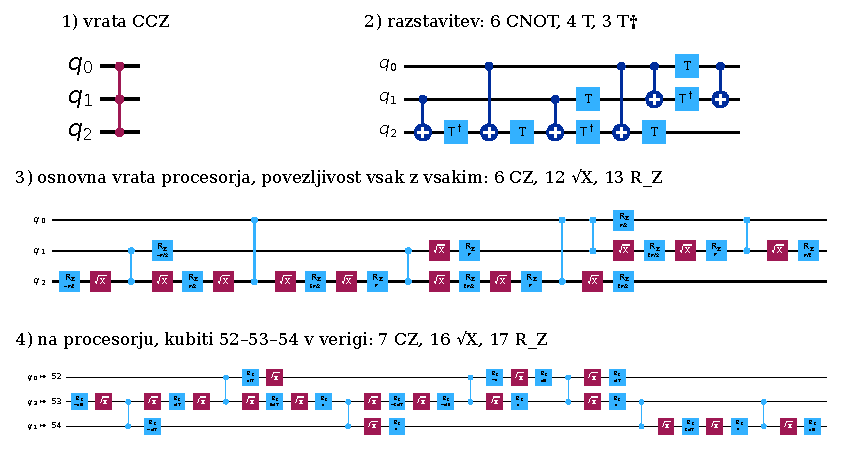
\includegraphics[height=0.80\textheight]{kaskada_ccz}
\end{frame}

% ---------------------------------------------------------------------
\begin{frame}{Prevajanje: število vrat hitro raste}
  \begin{columns}[c]
    \begin{column}{0.58\textwidth}
      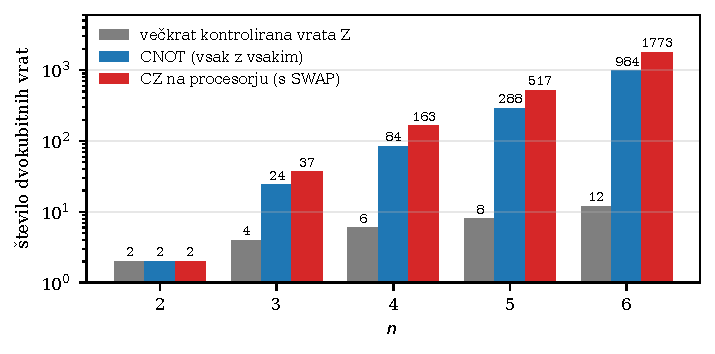
\includegraphics[width=\textwidth]{kaskada_n}
    \end{column}
    \begin{column}{0.40\textwidth}
      \begin{itemize}
        \item Procesor zna le CZ, $\sqrt{X}$, $X$ in $R_Z$.
        \item $CCZ$ $\to$ 6 CNOT, $C^5Z$ $\to$ 82 CNOT.
        \item Vsak kubit ima največ 3 sosede $\to$ vrata SWAP.
        \item Pri $n = 6$: \alert{\num{1773} vrat CZ} (stopnja 3).
      \end{itemize}
    \end{column}
  \end{columns}
\end{frame}

% ---------------------------------------------------------------------
\begin{frame}{Digitalni dvojčki in poskus}
  Vsi dvojčki: \texttt{NoiseModel.from\_backend} (Qiskit Aer) --- termična relaksacija ($T_1$, $T_2$), depolarizacija vrat in napaka odčitavanja.

  \vspace{0.6em}
  \centering
  \small
  \begin{tabular}{lll}
    \toprule
    Dvojček & Kalibracija & Čakanje kubitov \\
    \midrule
    živa kalibracija / CSV & posnetek ob prevajanju (enaka) & da \\
    FakeMarrakesh & stari posnetek (26.\,2.\,2025) & da \\
    brez čakanja (kontrola) & kot CSV & ne \\
    \bottomrule
  \end{tabular}

  \vspace{0.8em}
  \raggedright
  \normalsize
  \begin{itemize}
    \item Vezja za $n = 2\ldots6$ prevedena \alert{enkrat}; isto vezje gre na procesor in v vse dvojčke.
    \item 3 naloge na \texttt{ibm\_marrakesh}, vsaka 10 vezij $\times$ \num{10000} ponovitev.
  \end{itemize}
\end{frame}

% ---------------------------------------------------------------------
\begin{frame}{Rezultat: prag je pri $n^* = 6$}
  \begin{columns}[c]
    \begin{column}{0.64\textwidth}
      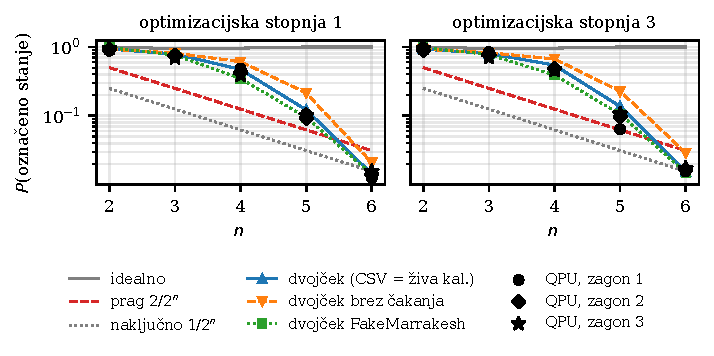
\includegraphics[width=\textwidth]{prag}
    \end{column}
    \begin{column}{0.34\textwidth}
      \begin{itemize}
        \item $n = 5$ ($\approx 520$ CZ): $P \approx \num{0,10}$, prag \num{0,0625}.
        \item $n = 6$ ($\approx \num{1800}$ CZ): $P \approx \num{0,016}$ = naključno ugibanje.
        \item Ponovi se v vseh treh nalogah.
        \item \alert{Vsi dvojčki} napovejo isti prag.
      \end{itemize}
    \end{column}
  \end{columns}
\end{frame}

% ---------------------------------------------------------------------
\begin{frame}{Dvojčki precenijo $P$ --- predvsem zaradi čakanja}
  \begin{columns}[c]
    \begin{column}{0.62\textwidth}
      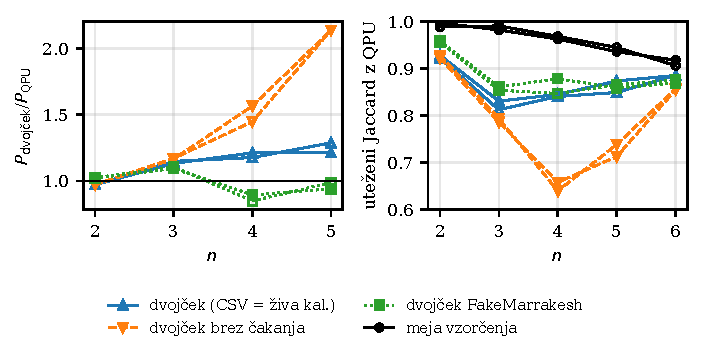
\includegraphics[width=\textwidth]{cakanje}
    \end{column}
    \begin{column}{0.36\textwidth}
      Precenitev pri $n = 5$:
      \begin{itemize}
        \item brez čakanja: \alert{\num{2,1}-krat}
        \item s čakanjem: \num{1,2}- do \num{1,3}-krat
      \end{itemize}
      \vspace{0.5em}
      Pri $n = 5$ kubiti čakajo \SIrange{71}{73}{\percent} časa vezja ($\approx \SI{40}{\micro\second}$ pri $T_2 \approx \SIrange{130}{240}{\micro\second}$).
    \end{column}
  \end{columns}
\end{frame}

% ---------------------------------------------------------------------
\begin{frame}{Je to hitreje od klasičnega iskanja?}
  Povprečno število poizvedb, da najdemo in preverimo označeni element:

  \vspace{0.6em}
  \centering
  \begin{tabular}{rrrr}
    \toprule
    $n$ & klasično $(N+1)/2$ & idealni Grover & Grover na procesorju \\
    \midrule
    2 & \num{2,5}  & \num{2,0} & \num{2,1} \\
    3 & \num{4,5}  & \num{3,2} & \num{4,3} \\
    4 & \num{8,5}  & \num{4,2} & \num{8,7} \\
    5 & \num{16,5} & \num{5,0} & \alert{\num{47,0}} \\
    6 & \num{32,5} & \num{7,0} & \alert{402} \\
    \bottomrule
  \end{tabular}

  \vspace{0.8em}
  \raggedright
  Na procesorju je Grover hitrejši od klasičnega iskanja \alert{le do $n = 3$}.
\end{frame}

% ---------------------------------------------------------------------
\begin{frame}{Zaključek}
  \begin{itemize}
    \item Groverjev algoritem na IBM Heron deluje do $n = 5$ in preneha pri \alert{$n^* = 6$} (med $\approx 500$ in $\approx \num{1800}$ vrati CZ).
    \item Dvojček iz kalibracijskih podatkov prag \alert{napove pravilno}, verjetnost uspeha pa preceni.
    \item Največji del precenitve pojasni dekoherenca kubitov med čakanjem; brez nje je model za napoved $P$ neuporaben.
    \item Prednost pred klasičnim iskanjem le do $n = 3$.
  \end{itemize}

  \vspace{0.8em}
  \textbf{Naprej:} orakelj s pomožnimi kubiti, presluh in koherentne napake v modelu.
\end{frame}

% ---------------------------------------------------------------------
\begin{frame}[standout]
  Hvala za pozornost!

  \vspace{0.5em}
  {\normalsize Vprašanja?}
\end{frame}

% =====================================================================
% Rezervne prosojnice (za vprašanja)
\appendix

\begin{frame}{Rezerva: izboljšava nad ugibanjem v odvisnosti od vrat CZ}
  \centering
  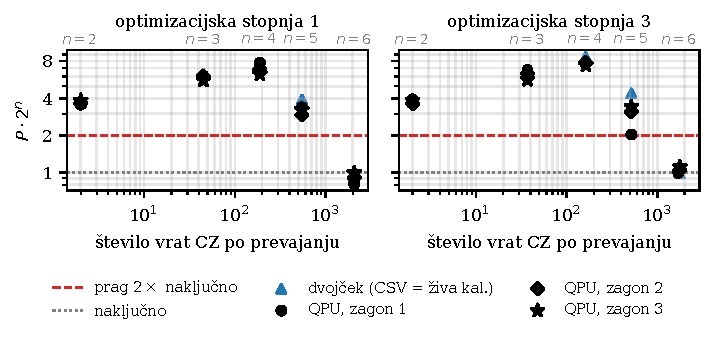
\includegraphics[height=0.72\textheight]{vrata}

  {\small Prag leži med $\approx 500$ in $\approx \num{1800}$ vrati CZ.}
\end{frame}

\begin{frame}{Rezerva: kaj ni delovalo}
  \begin{itemize}
    \item \textbf{Ročno zgrajen model iz CSV} je bil »pravilen iz napačnega razloga«: dekoherenco je štel dvakrat, čakanja pa ni upošteval; napaki sta se delno izničili.
    \item \textbf{Stopnja 3 brez skupne postavitve} je izbrala druge (slabše) kubite; primerjava stopenj je tako primerjala dele čipa. Od zagona 2 naprej imata stopnji isto postavitev.
    \item \textbf{Napačni kalibracijski podatki}: CSV z 21.\,11. je za kubita 0 in 1 navajal verjetnost napačnega odčitavanja stanja $\ket{0}$ \num{0,39} in \num{0,70}; dvojček je lahko le tako dober kot podatki.
  \end{itemize}
\end{frame}

\end{document}
